\documentclass[xcolor={usenames,svgnames}]{beamer}

\usepackage[english]{babel}
\usepackage{rtxslides}
\usepackage{listings}
\usepackage{tikz}
\usepackage{graphicx}
\usetikzlibrary{shapes,fit,positioning}

\lstdefinelanguage{rathaxes}%
{
	morekeywords={
        interface, extend,                      % interfaces : decl
        device, configuration, driver,          % devices
        with, values,                           % backend+interface
        builtin, provided, required, optional,  % interfaces: implem
        type, sequence, variable,               % general: element type
        pointcut, chunk,                        % for aspectual concepts
        template                                % backend
    },%
	morecomment=[l][\color{Gainsboro}]{//},%
 	morecomment=[l][\color{Gainsboro}]{\#},%
	morecomment=[s][\color{Gainsboro}]{/*}{*/},%
	morestring=[b][\color{Gold}]",%
	morestring=[b][\color{Gold}]',%
	keywordstyle={\color{Tomato}}%
}[keywords,comments,strings]

\lstset{
    language=rathaxes,
    tabsize=4,
    captionpos=b,
    emptylines=0,
    breaklines=false,
    breakatwhitespace=false,        % sets if automatic breaks should only happen at whitespace
    extendedchars=false,
    showstringspaces=false,
    showspaces=false,
    numbersep=1ex,
    showtabs=false,
    basicstyle=\color{white}\scriptsize\ttfamily,
    numberstyle=\color{Gainsboro}\scriptsize\ttfamily,
    stepnumber=1,                   % the step between two line-numbers. If it's 1, each line
    keywordstyle=\color{Tomato},
    commentstyle=\color{Gainsboro},
    stringstyle=\color{white},
    backgroundcolor=\color{black},
    escapeinside={\%*}{*)},         % if you want to add a comment within your code
    morekeywords={*,...}            % if you want to add more keywords to the set
}

\title{\rtx\ -- Gdt Programmation/IRILL 2012}
\date{October 25\textsuperscript{th} 2012}
\author{L. Auroux\\ \texttt{www.rathaxes.org}}

\definecolor{lightred}{RGB}{147,36,33}
\tikzset{componentarrow/.style={->, >=stealth, color=rathaxesred, ultra thick}}

\newcommand{\cemph}[1]{{\itshape{\textcolor{rathaxesred}{#1}}}}

\newcommand{\tred}[1]{\textcolor{rathaxesred}{#1}}

\tikzset{warrow/.style={->, >=stealth, color=white, ultra thick}}

\tikzset{graybox/.style={draw,rectangle,rounded corners=3pt,very thick,densely dashed,color=gray!75,text=white}}
\tikzset{redbox/.style={draw,rectangle,rounded corners=5pt,ultra thick,color=rathaxesred,text=white}}
\tikzset{redcontainer/.style={draw,rectangle,rounded corners=5pt,ultra thick,color=rathaxesred,text=white,minimum height=3.5cm,minimum width=2.5cm}}

\begin{document}

\begin{frame}
\titlepage
\end{frame}

\begin{frame}{Who am I?}
\begin{itemize}
\item EPITA-EPITECH Teachers;
\item Computer Fields: System, Security, Languages implementation;
\item leader of the Project Rathaxes.
\end{itemize}
\end{frame}

\begin{frame}{Plan}
\begin{itemize}
\item 1) Problematic
\item 2) Past Solutions?
\item 3) Our solutions
\item 4) Demos
\item 5) Open problems
\item 6) Conclusions/Questions
\end{itemize}
\end{frame}

\begin{frame}{Pre-requisites}
\begin{itemize}
\item Kernel: The Base Component of OSes;
\item Device: The Hardware/board plugged into the motherboard;
\item Subsystems: Abstraction layer for big computer features (Network, FS, Storage, USB, \ldots);
\item Driver: The software component loaded into the kernel.
\end{itemize}
\end{frame}

\begin{frame}{Drivers}
\begin{itemize}
\item A big amount of kernel code (ex:70 \% of linux kernel);
\item A critical amount of code (ex: BSOD);
\item A difficult to write amount of code (device specific VS Os specific).
\end{itemize}
\end{frame}

\begin{frame}[fragile]{What is a driver?}
\begin{tikzpicture}[overlay]
% User processes box and its text
\node[redbox, minimum height=6cm, minimum width=1.5cm] (USERLAND) at (0.7,-0.3) {};
    \node[]                       (ul) at (USERLAND.center) {l};
    \node[anchor=south]           (ur) at (ul.north)        {r};
    \node[anchor=south]           (ue) at (ur.north)        {e};
    \node[anchor=south]           (us) at (ue.north)        {s};
    \node[anchor=south]           (uu) at (us.north)        {U};
    \node[anchor=north]           (ua) at (ul.south)        {a};
    \node[anchor=north]           (un) at (ua.south)        {n};
    \node[anchor=north]           (ud) at (un.south)        {d};

%System box, invisible which contains KERNEL and DRIVER
\node[minimum height=6cm, minimum width=5cm, right=6mm] (SYSTEM) at (USERLAND.east) {};

    % Kernel box and its components
    \node[redbox, minimum height=4.2cm, minimum width=5cm, anchor=north] (KERNEL) at (SYSTEM.north) {};
    \draw (KERNEL.north) node [below]{\Large{Kernel}};
        \node[graybox, minimum height=4.0cm, minimum width=0.8cm, right=1mm, anchor=west] (KUSER) at (KERNEL.west) {};
            \node[anchor=north]             (kul) at (KUSER.center)  {l};
            \node[above=-1mm, anchor=south] (kur) at (kul.north)     {r};
            \node[above=-1mm, anchor=south] (kue) at (kur.north)     {e};
            \node[above=-1mm, anchor=south] (kus) at (kue.north)     {s};
            \node[above=-1mm, anchor=south] (kuu) at (kus.north)     {U};
            \node[below=-1mm, anchor=north] (kua) at (kul.south)     {a};
            \node[below=-1mm, anchor=north] (kun) at (kua.south)     {n};
            \node[below=-1mm, anchor=north] (kud) at (kun.south)     {d};
        \node[graybox, minimum height=1.8cm, minimum width=1cm] (VFS) at (KERNEL.center) {};
            \node[]                 (vf) at (VFS.center) {F};
            \node[anchor=south]     (vv) at (vf.north)   {V};
            \node[anchor=north]     (vs) at (vf.south)   {S};
        \node[graybox, minimum height=1.8cm, minimum width=1cm, right=5mm] (NET) at (VFS.east) {};
            \node[]                 (ne) at (NET.center) {E};
            \node[anchor=south]     (nn) at (ne.north)   {N};
            \node[anchor=north]     (nt) at (ne.south)   {T};

    % Driver box and its components
    \node[redbox, minimum height=1.6cm, minimum width=5cm, anchor=south] (DRIVER) at (SYSTEM.south) {};
    \draw (DRIVER.south) node [above]{\Large{Driver}};
        \node[graybox, minimum height=0.7cm, minimum width=4.8cm, anchor=south] (ALGO) at (DRIVER.center) {Algorithms};

% BUS box and its texts
\node[redbox, minimum height=6cm, minimum width=15mm, right=4mm] (BUS) at (SYSTEM.east) {};
    \draw (BUS.north) node [below]{\Large{BUS}};
    \node[graybox       ] (PCI) at (BUS.center) {PCI};
    \node[graybox, above=2mm of PCI] (USB) at (PCI.north)  {USB};
    \node[graybox, below=2mm of PCI] (ISA) at (PCI.south)  {ISA};
    \node[graybox, below=2mm of ISA, minimum height=1em] (I2C) at (ISA.south)  {\ldots};

% Register box and its text
\node[graybox, minimum width=5cm, minimum height=8mm, rotate=90, right=7mm, anchor=north] (REGISTERS) at (BUS.east) {};
    \node[            ]  (rs1) at (REGISTERS.center) {s};
    \node[anchor=south]  (ri)  at (rs1.north)        {i};
    \node[anchor=south]  (rg)  at (ri.north)         {g};
    \node[anchor=south]  (re1) at (rg.north)         {e};
    \node[anchor=south]  (rr1) at (re1.north)        {R};
    \node[anchor=north]  (rt)  at (rs1.south)        {t};
    \node[anchor=north]  (re2) at (rt.south)         {e};
    \node[anchor=north]  (rr2) at (re2.south)        {r};
    \node[anchor=north]  (rs2) at (rr2.south)        {s};

% Peripherals box and its text
\node[redbox,minimum width=6cm,minimum height=1cm, rotate=90, below=0mm] (DEV) at (REGISTERS.south) { };
    \node[            ]  (ph)  at (DEV.center) {h};
    \node[anchor=south]  (pp2) at (ph.north)   {p};
    \node[anchor=south]  (pi)  at (pp2.north)  {i};
    \node[anchor=south]  (pr1) at (pi.north)   {r};
    \node[anchor=south]  (pe1) at (pr1.north)  {e};
    \node[anchor=south]  (pp1) at (pe1.north)  {P};
    \node[anchor=north]  (pe2) at (ph.south)   {e};
    \node[anchor=north]  (pr2) at (pe2.south)  {r};
    \node[anchor=north]  (pa)  at (pr2.south)  {a};
    \node[anchor=north]  (pl)  at (pa.south)   {l};
    \node[anchor=north]  (ps)  at (pl.south)   {s};

\end{tikzpicture}
\end{frame}

\begin{frame}{Driver anatomy}
\begin{itemize}
\item Low-level Part:
\begin{itemize}
\item Device dependent registers/descriptors;
\item Board dependent buses;
\item Objectives: Abstraction of Registers/Descriptors access thru Buses.
\end{itemize}
\item High-level Part:
\begin{itemize}
\item Device independent logic using low-level part;
\item Kernel dependent subsytems API;
\item Objectives: Use kernel abstraction to interface device logic with kernel subsystems.
\end{itemize}
\end{itemize}
\end{frame}

\begin{frame}{Solutions?}
\begin{itemize}
\item Basic abstraction layer:
\begin{itemize}
\item All open source kernels...
\end{itemize}
\item Abstraction layer + tools:
\begin{itemize}
\item WDF (Windows Driver Frameworks) + Static Driver Verifier Research Platform: check API compliance with model checking
\item Safedriver (Linux) : Source-to-Source transformation tool (autoinsertion of validity check, use kernel header annotation)
\end{itemize}
\item Automated tools:
\begin{itemize}
\item Windriver: Multi-Os (windowses, linux), User mode
\end{itemize}
\end{itemize}
\end{frame}

\begin{frame}[fragile]{Solutions?}
\begin{itemize}
\item IDL (Interface Description Language):
\begin{itemize}
\item Devil: 2002, L. Reveillere (Linux only)
\item HAIL: 2005, J.Sun,W.Yuan,M.Kallahalla (Linux, netbsd)
\end{itemize}
\begin{center}
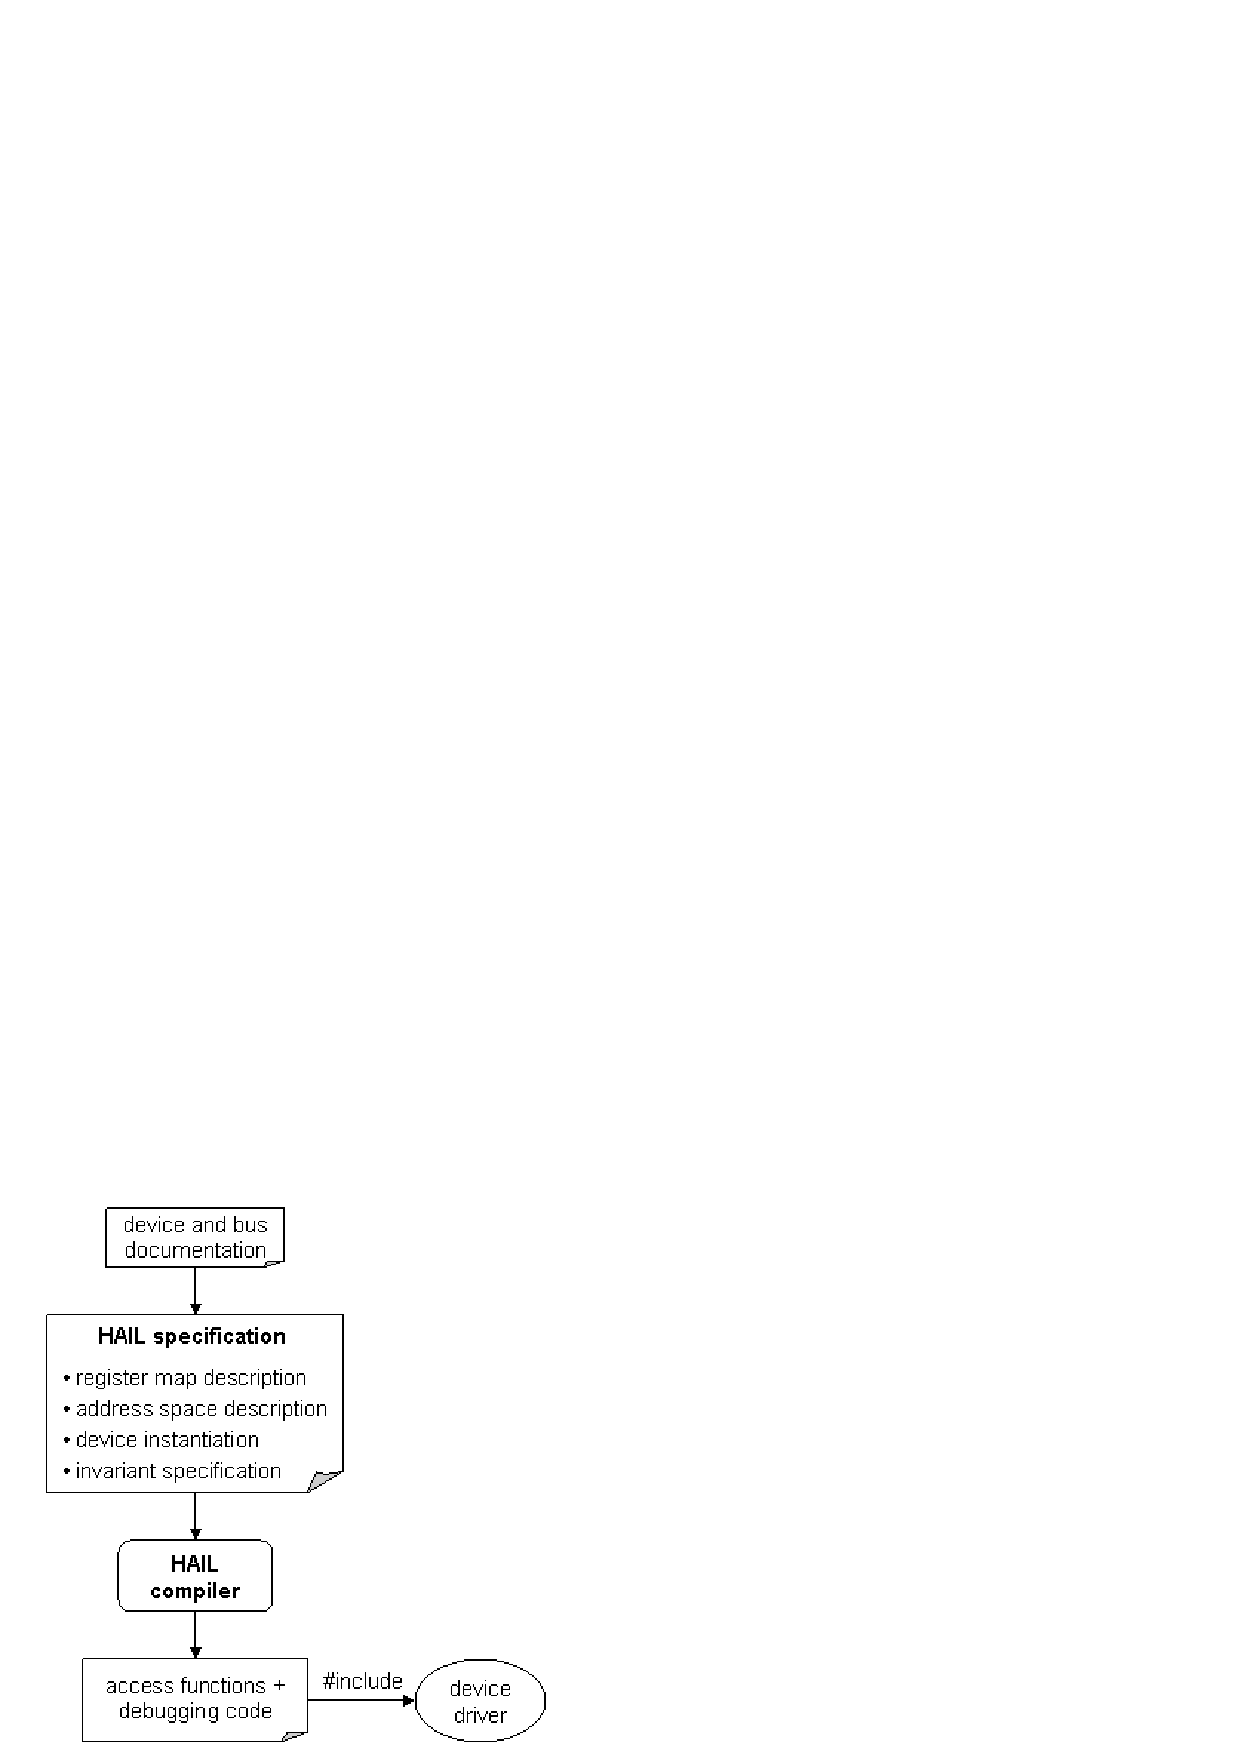
\includegraphics[scale=0.5,viewport=1 100 600 260]{hail_overview.pdf}
\end{center}
\end{itemize}
\end{frame}

\begin{frame}{Critics}
\begin{itemize}
\item Pros
\begin{itemize}
\item Register mapping (logical check)
\item Code generation safety
\end{itemize}
\item Cons
\begin{itemize}
\item Few Oses
\item No control of Kernel dependent code
\item Only Low-level part of driver
\end{itemize}
\end{itemize}
\end{frame}

\begin{frame}{Solutions?}
\begin{itemize}
\item DSL (Domain Specific Language):
\begin{itemize}
\item NDL: 2004, C.Conway (University columbia)
\item Termite: 2009, Open kernel Labs
\end{itemize}
\end{itemize}
\end{frame}

\begin{frame}{Critics}
\begin{itemize}
\item Pros
\begin{itemize}
\item Specialized for a device familly (NDL)
\item Full description for termite
\end{itemize}
\item Cons
\begin{itemize}
\item Nothing to download (NDL or Termite)
\item Business company: Open Kernel Lab
\end{itemize}
\end{itemize}
\end{frame}

\begin{frame}{Our Solution}
\begin{itemize}
\item DSL able to describe all device component (independent, dependent);
\item Full open source solution;
\item Allow control of Kernel dependent code generation (template oriented).
\end{itemize}
\end{frame}

\begin{frame}{Our Solution}
How?
\begin{itemize}
\item Separation of concern, 3 use cases
\begin{itemize}
\item Kernel programmer
\item Device programmer
\item Rathaxes programmer
\end{itemize}
\item So one language in 3 part
\begin{itemize}
\item A Middle-end language, able to describe compiler semantics
\item A Back-end language, able to manipulate chunks of C code
\item A Front-end language, able to instanciate all the stuff
\end{itemize}
\end{itemize}
\end{frame}

\begin{frame}{\rtx\ language (Middle-End)}
\begin{tikzpicture}[overlay]
\node (RTI) at (1.2,0) {
\includegraphics[height=1.5cm]{icons/rti}};

\draw (RTI.north east) node[below right]{%
    \begin{minipage}{10cm}
    Describe \emph{``subsystems''} with:
    \begin{itemize}
    \item Types;
    \item Sequences;
    \item Configuration variables;
    \end{itemize}
    \end{minipage}
};
\end{tikzpicture}
\end{frame}

\begin{frame}[fragile]{\rtx\ language (Middle-End)}
\begin{tikzpicture}[overlay]
\node (RTI) at (1.2,0) {
\includegraphics[height=1.5cm]{icons/rti}};

\draw (RTI.east) node[right]{%
    \begin{minipage}{10cm}
    \begin{lstlisting}
    interface CharDev : LKM {
      provided type        Context;
      required sequence    open(Context) {
         provided chunk    LKM::GLOBAL_CODE_DEFINITION;
         provided chunk    LKM::INIT_LKM_FPTRS;
         provided pointcut ALGO;
      }
      required variable identifier  OS;
      required variable serial      version;
    }
    \end{lstlisting}
    \end{minipage}
};
\end{tikzpicture}
\end{frame}


\begin{frame}{\rtx\ language (Back-End)}
\begin{tikzpicture}[overlay]
\node (BLT) at (1.2,0) {
\includegraphics[height=1.5cm]{icons/blt}};

\draw (BLT.north east) node[below right]{%
    \begin{minipage}{10cm}
        Implement the interfaces for each OS:
        \begin{itemize}
        \item Types templates;
        \item Sequences templates.
        \end{itemize}
    \end{minipage}
};
\end{tikzpicture}
\end{frame}

\begin{frame}[fragile]{\rtx\ language (Back-End)}
\begin{tikzpicture}[overlay]
\node (BLT) at (1.2,0) {
\includegraphics[height=1.5cm]{icons/blt}};

\draw (BLT.east) node[right]{%
    \begin{minipage}{10cm}
    \begin{lstlisting}
    with CharDev
    values OS = Linux, version >= 2.6.27 {
      template sequence CharDev::open(Context ctx) {
         chunk LKM::INIT_LKM_FPTRS() {
             /* Instrumentalized C */
             .open = &${self.devname}_write
         }
         chunk ::CALL() {
                int     ${self.devname}_write(dev_t *ctx)
                {/*....*/}
         }
      }
    }
    \end{lstlisting}
    \end{minipage}
};
\end{tikzpicture}
\end{frame}


\begin{frame}{\rtx\ language (Front-End)}
\begin{tikzpicture}[overlay]
\node (RTX) at (1.2,0) {
\includegraphics[height=1.5cm]{icons/rtx}};

\draw (RTX.north east) node[below right]{%
    \begin{minipage}{10cm}
        Hardware, algorithms and target descriptions:
        \begin{itemize}
        \item Registers;
        \item Sequences' algorithms;
        \item Configuration.
        \end{itemize}
    \end{minipage}
};
\end{tikzpicture}
\end{frame}

\begin{frame}[fragile]{\rtx\ language (Back-End)}
\begin{tikzpicture}[overlay]
\node (RTX) at (1.2,0) {
\includegraphics[height=1.5cm]{icons/rtx}};

\draw (RTX.east) node[right]{%
    \begin{minipage}{115mm}
    \begin{lstlisting}
    device Pipe use LKM, CharDev, Algorithms {
        register byte APR mode RW like (*****...) at 3
        {
            [0..1] as word_lengh {
                (00) -> _5bits;
                (01) -> _6bits;
                (10) -> _7bits;
                (11) -> _8bits;
            }
            [2] as stop_bits {
                (0) -> _1stop_bits;
                (1) -> _2stop_bits;
            }
        }
      open(Context ctx) {
         Generic::log("Open called on device!");
         Generic::set(APR->word_lengh._7bits);
         log("initialized"); // unqualified call
      }
    }
    \end{lstlisting}
    \end{minipage}
};
\end{tikzpicture}
\end{frame}


\begin{frame}[fragile]{Interactions between the language parts}
\begin{tikzpicture}[overlay]
\node (RTX) at (1.2,2.4) {
\includegraphics[height=1.5cm]{icons/rtx}};
\draw (RTX.east) node[right]{%
\begin{minipage}{115mm}
\begin{lstlisting}
device Pipe use LKM, CharDev, Algorithms {
  open(Context ctx) {
     log("Open called on device Pipe");
  }
}
\end{lstlisting}
\end{minipage}};

\node (RTI) at (1.2,-0.1) {
\includegraphics[height=1.5cm]{icons/rti}};

\draw (RTI.east) node[right]{%
\begin{minipage}{115mm}
\begin{lstlisting}
interface CharDev : LKM {
  provided type        Context;
  required sequence    open(Context) {
     provided chunk    LKM::GLOBAL_CODE_DEFINITION;
     provided chunk    LKM::INIT_LKM_FPTRS;
     provided pointcut ALGO;
  }
  required variable identifier  OS;
  required variable serial      version;
}
\end{lstlisting}
\end{minipage}};

\node (BLT) at (1.2,-3.2) {
\includegraphics[height=1.5cm]{icons/blt}};

\draw (BLT.east) node[right]{%
\begin{minipage}{115mm}
\begin{lstlisting}
with CharDev
values OS = Linux, version >= 2.6.27 {
  template sequence CharDev::open(Context ctx) {
     chunk LKM::GLOBAL_CODE_DEFINITION {
         ${pointcut ALGO}
     }
  }
}
\end{lstlisting}
\end{minipage}};
\end{tikzpicture}
\end{frame}

\begin{frame}[fragile]{Interactions between the language parts}
\begin{tikzpicture}[overlay]
\node (RTX) at (1.2,2.4) {
\includegraphics[height=1.5cm]{icons/rtx}};
\draw (RTX.east) node[right]{%
\begin{minipage}{115mm}
\begin{lstlisting}
device Pipe use LKM, CharDev, Algorithms {
  open(Context ctx) {
     log("Open called on device Pipe");
  }
}
\end{lstlisting}
\end{minipage}};

\node (RTI) at (1.2,-0.1) {
\includegraphics[height=1.5cm]{icons/rti}};

\draw (RTI.east) node[right]{%
\begin{minipage}{115mm}
\begin{lstlisting}
interface CharDev : LKM {
  provided type        Context;
  required sequence    open(Context) {
     provided chunk    LKM::GLOBAL_CODE_DEFINITION;
     provided chunk    LKM::INIT_LKM_FPTRS;
     provided pointcut ALGO;
  }
  required variable identifier  OS;
  required variable serial      version;
}
\end{lstlisting}
\end{minipage}};

\node (BLT) at (1.2,-3.2) {
\includegraphics[height=1.5cm]{icons/blt}};

\draw (BLT.east) node[right]{%
\begin{minipage}{115mm}
\begin{lstlisting}
with CharDev
values OS = Linux, version >= 2.6.27 {
  template sequence CharDev::open(Context ctx) {
     chunk LKM::GLOBAL_CODE_DEFINITION {
         ${pointcut ALGO}
     }
  }
}
\end{lstlisting}
\end{minipage}};
\draw [ultra thick, rounded corners=3pt, color=DodgerBlue] (2.47,-0.74) rectangle (8.22,-1.1);
\draw [ultra thick, color=DodgerBlue, ->, >=stealth] (5.5,-1.1) -- (3.7,-2.19);
\end{tikzpicture}
\end{frame}

\begin{frame}[fragile]{Interactions between the language parts}
\begin{tikzpicture}[overlay]
\node (RTX) at (1.2,2.4) {
\includegraphics[height=1.5cm]{icons/rtx}};
\draw (RTX.east) node[right]{%
\begin{minipage}{115mm}
\begin{lstlisting}
device Pipe use LKM, CharDev, Algorithms {
  open(Context ctx) {
     log("Open called on device Pipe");
  }
}
\end{lstlisting}
\end{minipage}};

\node (RTI) at (1.2,-0.1) {
\includegraphics[height=1.5cm]{icons/rti}};

\draw (RTI.east) node[right]{%
\begin{minipage}{115mm}
\begin{lstlisting}
interface CharDev : LKM {
  provided type        Context;
  required sequence    open(Context) {
     provided chunk    LKM::GLOBAL_CODE_DEFINITION;
     provided chunk    LKM::INIT_LKM_FPTRS;
     provided pointcut ALGO;
  }
  required variable identifier  OS;
  required variable serial      version;
}
\end{lstlisting}
\end{minipage}};

\node (BLT) at (1.2,-3.2) {
\includegraphics[height=1.5cm]{icons/blt}};

\draw (BLT.east) node[right]{%
\begin{minipage}{115mm}
\begin{lstlisting}
with CharDev
values OS = Linux, version >= 2.6.27 {
  template sequence CharDev::open(Context ctx) {
     chunk LKM::GLOBAL_CODE_DEFINITION {
         ${pointcut ALGO}
     }
  }
}
\end{lstlisting}
\end{minipage}};
\draw [ultra thick, rounded corners=3pt, color=DodgerBlue] (2.47,-0.74) rectangle (8.22,-1.1);
\draw [ultra thick, color=DodgerBlue, ->, >=stealth] (5.5,-1.1) -- (3.7,-2.19);

\draw [ultra thick, rounded corners=3pt, color=LimeGreen] (2.50,0.90) rectangle (8.3,0.55);
\draw [ultra thick, color=LimeGreen, ->, >=stealth] (6.80,0.90) -- (2.9,2.6);
\draw [ultra thick, color=LimeGreen, ->, >=stealth] (6.80,0.55) -- (7.45,-2.50);

\end{tikzpicture}
\end{frame}

\begin{frame}[fragile]{Interactions between the language parts}
\begin{tikzpicture}[overlay]
\node (RTX) at (1.2,2.4) {
\includegraphics[height=1.5cm]{icons/rtx}};
\draw (RTX.east) node[right]{%
\begin{minipage}{115mm}
\begin{lstlisting}
device Pipe use LKM, CharDev, Algorithms {
  open(Context ctx) {
     log("Open called on device Pipe");
  }
}
\end{lstlisting}
\end{minipage}};

\node (RTI) at (1.2,-0.1) {
\includegraphics[height=1.5cm]{icons/rti}};

\draw (RTI.east) node[right]{%
\begin{minipage}{115mm}
\begin{lstlisting}
interface CharDev : LKM {
  provided type        Context;
  required sequence    open(Context) {
     provided chunk    LKM::GLOBAL_CODE_DEFINITION;
     provided chunk    LKM::INIT_LKM_FPTRS;
     provided pointcut ALGO;
  }
  required variable identifier  OS;
  required variable serial      version;
}
\end{lstlisting}
\end{minipage}};

\node (BLT) at (1.2,-3.2) {
\includegraphics[height=1.5cm]{icons/blt}};

\draw (BLT.east) node[right]{%
\begin{minipage}{115mm}
\begin{lstlisting}
with CharDev
values OS = Linux, version >= 2.6.27 {
  template sequence CharDev::open(Context ctx) {
     chunk LKM::GLOBAL_CODE_DEFINITION {
         ${pointcut ALGO}
     }
  }
}
\end{lstlisting}
\end{minipage}};
\draw [ultra thick, rounded corners=3pt, color=DodgerBlue] (2.47,-0.74) rectangle (8.22,-1.1);
\draw [ultra thick, color=DodgerBlue, ->, >=stealth] (5.5,-1.1) -- (3.7,-2.19);

\draw [ultra thick, rounded corners=3pt, color=LimeGreen] (2.50,0.90) rectangle (8.3,0.55);
\draw [ultra thick, color=LimeGreen, ->, >=stealth] (6.80,0.90) -- (2.9,2.6);
\draw [ultra thick, color=LimeGreen, ->, >=stealth] (6.80,0.55) -- (7.45,-2.50);

\draw [ultra thick, rounded corners=3pt, color=MediumOrchid] (3,-0.09) rectangle (7,-0.43);
\draw [ultra thick, color=MediumOrchid, ->, >=stealth] (5.8,-0.09) -- (5,2.27);
\draw [ultra thick, color=MediumOrchid, ->, >=stealth] (5.8,-0.41) -- (5,-3.22);
\end{tikzpicture}
\end{frame}

\begin{frame}{Driver generation work-flow}
\only<1>{\begin{tikzpicture}[overlay]
\node (RTX) at (3.5,2.5) {
\includegraphics[height=1.5cm]{icons/rtx}};
\node[redbox] (COMPILER) at (3.5,-0.5) {Compiler};
\node (C) at (3.5,-3.5) {
\includegraphics[height=1.5cm]{icons/c}};

\draw[warrow] (RTX)--(COMPILER);
\draw[warrow] (COMPILER)--(C);

\draw (RTX.north east) node[below right]{\large{Driver description}};
\draw (C.north east) node [below right]{\large{Kernel module}};
\end{tikzpicture}}

\only<2>{\begin{tikzpicture}[overlay]
\node[opacity=0.3] (RTX) at (3.5,2.5) {
\includegraphics[height=1.5cm]{icons/rtx}};
\node[redcontainer] (COMPILER) at (3.5,-0.5) {};
\node[opacity=0.3] (C) at (3.5,-3.5) {
\includegraphics[height=1.5cm]{icons/c}};

\draw[warrow,opacity=0.3] (RTX)--(COMPILER);
\draw[warrow,opacity=0.3] (COMPILER)--(C);

\draw (RTX.north east) node[below right, opacity=0.3]{\large{Driver description}};
\draw (COMPILER.south east) node[above right]{\Large{Compiler}};
\draw (C.north east) node [below right, opacity=0.3]{\large{Kernel module}};
\end{tikzpicture}}

\only<3>{\begin{tikzpicture}[overlay]
\node[opacity=0.3] (RTX) at (3.5,2.5) {
\includegraphics[height=1.5cm]{icons/rtx}};
\draw (RTX.north east) node[below right, opacity=0.3]{\large{Driver description}};

\node[opacity=0.3] (C) at (3.5,-3.5) {
\includegraphics[height=1.5cm]{icons/c}};

\node[graybox] (AST1) at (3.5,0.5){\texttt{AST}};
\draw[warrow] (RTX)--(AST1);

%\node[graybox] (AST2) at (3.5,-1.5) {\texttt{AST}};
%\draw[warrow] (AST2)--(C);

\node[redcontainer] (COMPILER) at (3.5,-0.5) {};
\draw (COMPILER.south east) node[above right]{\Large{Compiler}};

%\node[graybox] (RTXLINK) at (COMPILER.center) {\texttt{RTX\_Link}};
%\draw[warrow] (AST1)--(RTXLINK);
%\draw[warrow] (RTXLINK)--(AST2);

\draw[warrow,opacity=0.3] (COMPILER)--(C);
\draw (C.north east) node [below right, opacity=0.3]{\large{Kernel module}};
\end{tikzpicture}}

\only<4>{\begin{tikzpicture}[overlay]
\node[opacity=0.3] (RTX) at (3.5,2.5) {
\includegraphics[height=1.5cm]{icons/rtx}};
\draw (RTX.north east) node[below right, opacity=0.3]{\large{Driver description}};

\node[opacity=0.3] (C) at (3.5,-3.5) {
\includegraphics[height=1.5cm]{icons/c}};

\node[graybox] (AST1) at (3.5,0.5){\texttt{AST}};
\draw[warrow] (RTX)--(AST1);

%\node[graybox] (AST2) at (3.5,-1.5) {\texttt{AST}};
%\draw[warrow] (AST2)--(C);

\node[redcontainer] (COMPILER) at (3.5,-0.5) {};
\draw (COMPILER.south east) node[above right]{\Large{Compiler}};

\node[graybox] (RTXLINK) at (COMPILER.center) {\texttt{RTX\_Link}};
\draw[warrow] (AST1)--(RTXLINK);
%\draw[warrow] (RTXLINK)--(AST2);

\draw[warrow,opacity=0.3] (COMPILER)--(C);
\draw (C.north east) node [below right, opacity=0.3]{\large{Kernel module}};
\end{tikzpicture}}

\only<5>{\begin{tikzpicture}[overlay]
\node[opacity=0.3] (RTX) at (3.5,2.5) {
\includegraphics[height=1.5cm]{icons/rtx}};
\draw (RTX.north east) node[below right, opacity=0.3]{\large{Driver description}};

\node[opacity=0.3] (C) at (3.5,-3.5) {
\includegraphics[height=1.5cm]{icons/c}};

\node[graybox] (AST1) at (3.5,0.5){\texttt{AST}};
\draw[warrow] (RTX)--(AST1);

%\node[graybox] (AST2) at (3.5,-1.5) {\texttt{AST}};
%\draw[warrow] (AST2)--(C);

\node[redcontainer] (COMPILER) at (3.5,-0.5) {};
\draw (COMPILER.south east) node[above right]{\Large{Compiler}};

\node[graybox] (RTXLINK) at (COMPILER.center) {\texttt{RTX\_Link}};
\draw[warrow] (AST1)--(RTXLINK);
%\draw[warrow] (RTXLINK)--(AST2);

\draw[warrow,opacity=0.3] (COMPILER)--(C);

\node (RTI) at (6,0.85) {
\includegraphics[height=1.3cm]{icons/rti}};
\draw (RTI.east) node[above right]{\Large{Interfaces}};
\draw[warrow] (RTI.west)--(RTXLINK.north);
\draw (C.north east) node [below right, opacity=0.3]{\large{Kernel module}};
\end{tikzpicture}}

\only<6>{\begin{tikzpicture}[overlay]
\node[opacity=0.3] (RTX) at (3.5,2.5) {
\includegraphics[height=1.5cm]{icons/rtx}};
\draw (RTX.north east) node[below right, opacity=0.3]{\large{Driver description}};

\node[opacity=0.3] (C) at (3.5,-3.5) {
\includegraphics[height=1.5cm]{icons/c}};

\node[graybox] (AST1) at (3.5,0.5){\texttt{AST}};
\draw[warrow] (RTX)--(AST1);

%\node[graybox] (AST2) at (3.5,-1.5) {\texttt{AST}};
%\draw[warrow] (AST2)--(C);

\node[redcontainer] (COMPILER) at (3.5,-0.5) {};
\draw (COMPILER.south east) node[above right]{\Large{Compiler}};

\node[graybox] (RTXLINK) at (COMPILER.center) {\texttt{RTX\_Link}};
\draw[warrow] (AST1)--(RTXLINK);
%\draw[warrow] (RTXLINK)--(AST2);

\draw[warrow,opacity=0.3] (COMPILER)--(C);

\node (RTI) at (6,0.85) {
\includegraphics[height=1.3cm]{icons/rti}};
\draw (RTI.east) node[above right]{\Large{Interfaces}};
\draw[warrow] (RTI.west)--(RTXLINK.north);

\node (BLT) at (6,-0.5) {
\includegraphics[height=1.3cm]{icons/blt}};
\draw (BLT.east) node[above right]{\Large{Code templates}};
\draw[warrow] (BLT.west)--(RTXLINK);
\draw (C.north east) node [below right, opacity=0.3]{\large{Kernel module}};
\end{tikzpicture}}

\only<7>{\begin{tikzpicture}[overlay]
\node[opacity=0.3] (RTX) at (3.5,2.5) {
\includegraphics[height=1.5cm]{icons/rtx}};
\draw (RTX.north east) node[below right, opacity=0.3]{\large{Driver description}};

\node[opacity=0.3] (C) at (3.5,-3.5) {
\includegraphics[height=1.5cm]{icons/c}};

\node[graybox] (AST1) at (3.5,0.5){\texttt{AST}};
\draw[warrow] (RTX)--(AST1);

\node[graybox] (AST2) at (3.5,-1.5) {\texttt{AST}};
\draw[warrow] (AST2)--(C);

\node[redcontainer] (COMPILER) at (3.5,-0.5) {};
\draw (COMPILER.south east) node[above right]{\Large{Compiler}};

\node[graybox] (RTXLINK) at (COMPILER.center) {\texttt{RTX\_Link}};
\draw[warrow] (AST1)--(RTXLINK);
\draw[warrow] (RTXLINK)--(AST2);

\node (RTI) at (6,0.85) {
\includegraphics[height=1.3cm]{icons/rti}};
\draw (RTI.east) node[above right]{\Large{Interfaces}};
\draw[warrow] (RTI.west)--(RTXLINK.north);

\node (BLT) at (6,-0.5) {
\includegraphics[height=1.3cm]{icons/blt}};
\draw (BLT.east) node[above right]{\Large{Code templates}};
\draw[warrow] (BLT.west)--(RTXLINK);
\draw (C.north east) node [below right, opacity=0.3]{\large{Kernel module}};
\end{tikzpicture}}
\end{frame}

\begin{frame}{}%First steps into \rtx}
	\begin{center}
	\Huge{\emph{Demonstration}}
	\end{center}
\end{frame}


\begin{frame}{Current state of \rtx}
        \Large{%
    \begin{center}
        \begin{itemize}
            \item 2002: L. Reveillere thesis \emph{``Devil''};
            \item 2007: Beginning of the project by a first team of EPITECH students;
            \item 2010-12: Refactoring/Improvement by a second team of EPITECH students, open sourcing;
            \item 2012: Rewriting codeworker/cnorm -> ???.
        \end{itemize}
    \end{center}
        }
\end{frame}

\begin{frame}{Open Problems}
    \begin{center}
        \Large{%
	\begin{itemize}
            \item Operationnal semantics of RTX|RTI;
            \item Operationnal semantic of BLT with C templates;
            \item Improvement of front-end DSL (interface/driver/kernel library);
            \item Test Environment (dummy peripherals).
	\end{itemize}
        }
    \end{center}
\end{frame}

\begin{frame}{Questions?}
\begin{center}
\Huge{Thanks}

\end{center}

%\hspace{1em}\rule{5cm}{0.2mm}
\vspace{2em}
\begin{itemize}
\item \Large{\texttt{http://www.rathaxes.org/}}
\item \Large{\texttt{\#rathaxes} on IRC (\texttt{irc.freenode.net})}
\end{itemize}
\end{frame}

\end{document}
